\documentclass{article}
\usepackage{graphicx}
\usepackage{subcaption}
\usepackage{geometry}
\usepackage{tikz}
\usepackage{amsmath}
\usepackage{cleveref}
\usepackage{float}
\usepackage[useregional]{datetime2}
\usepackage{url}
\def\checkmark{\tikz\fill[scale=0.4](0,.35) -- (.25,0) -- (1,.7) -- (.25,.15) -- cycle;}
\usepackage[font=small,skip=0pt]{caption}
\geometry{legalpaper, margin=1in}
\title{A Shallow Study on Rumble Strips' Effectiveness on Different Road Conditions}
\author{Zhijia Chen}
\date{\today}

\begin{document}

\begin{titlepage}
    \maketitle
\end{titlepage}

\section*{Summary}
Rumble strips has been widely adopted as an economic measure to alert inattentive drivers of potential dangers. A rumble strip is a raised or grooved pattern on travel lanes and has different texture with the road on with it is installed. When vehicle tires pass over the strip, they produce a sudden rumbling sound and cause the automobile to vibrate so as to alert inattentive or drowsy drivers\cite{corkle2001synthesis}. It is expected that drivers will pay more attention when passing the road and thus reduce the possibility of potential car accidents. A car accident is such a complex random event that contributed by many factors, it is hard to tell how effective rumble strips are in reducing crashes. So, in this study, we explore the effectiveness of rumble strips by comparing the changes in yearly car crashes number between roads with and without rumble installed in an observed time span (2004 to 2012). We find that there isn't strong evidence that rumble stripes have a general effects in reducing average number of crash on all roads. But when we focus on roads with certain condition, such as road curvature, road width, speed limit, etc., we found that on roads with curvature degree greater than 5, rumble strips can reduce the number of car crashes by 0.272 on average. We also find that rumble strips is likely to reduce 0.168 of car crashes on roads of width greater than 24 feet while they do not show positive effects in narrower roads, which is unexpected as by intuition we think a crash is more likely to happen if the road is narrower. By further investing the annual traffic volume, we realize that wider roads usually carry more traffic volume and thus higher car accident possibility, and that makes the effects of rumble strips more prominent.

\section*{Dataset and Assumption}

This study works with the dataset "PennCrash.txt"\cite{data} that provides number of crashes occurred on about 2000 road segments (sites) in Pennsylvania in the year 2004, 2008 and 2012. Among these sites, rumble strips were installed in 331 of them between year 2008 and 2012. The dataset also gives some features of the roads including annual average daily traffic (AADT) volume, curvature, width, posted speed limit and so on. As we do not know if rumble stripes were installed in 2008 or not, we only use the data of the year 2004 and 2012, and we assume that by the beginning of 2012, all the rumble stripes in this dataset had been installed. Thus we have a clean data to study the crash number before and after rumble strips installation.

\section*{Methodology}

To study if rumble strips help in reducing the number of car crashes, a naive approach is to compare the car accident number before and after rumble strip installation. However, 8 years (2004 to 2012) is quite a long time span and many factors that affect car crash could have changed over time, such as better traffic control system, improved overall driving behavior, better car control system, higher/lower traffic volume, etc., and we cannot simply ascribe the changes in car crashes to rumble stripes. So we take the sample of roads that do not have rumble strips treatment as a control group, and those that have rumble strips treatment as treat group. We will study the total crash number changes between year 2012 and year 2004 of the two groups, and test the differences between the two population. When investigating rumble strips' effects on roads with particular features, we will filter the data using the corresponding column before testing the differences. 

And to compare two population, we perform single-tailed two sample t-test to test if their means are equal and get the p value\cite{t-test}. Generally, we have the following null hypothesis and alternative hypothesis:

\begin{align*}
    H_0: &Mean(tot12-tot04)|(treat, condition(f_1, f_2, ..., f_n)) >= \\
         &Mean(tot12-tot04)|(not treat, condition(f_1, f_2, ..., f_n))\\
    H_1: &Mean(tot12-tot04)|(treat, condition(f_1, f_2, ..., f_n)) < \\
         &Mean(tot12-tot04)|(not treat, condition(f_1, f_2, ..., f_n))\\
\end{align*}

Where $tot04$ and $tot12$ are the total number of crashes in year 2004 and 2012 respectively, and $Mean(tot12-tot04)|(treat, condition(f_1, f_2, ..., f_n))$ denotes the mean value of $tot12-tot04$ of roads that have rumble stripe treatment with conditions on road features $f_1, f_2, ..., f_n$. $H_0$ means rumble strips treatment has no effect or has reverse effect in reducing car crash number on roads with features satisfying $condition(f_1, f_2, ..., f_n)$. We set $\alpha$ value to 0.05 in this study.

\section*{Exploratory Data Analysis}

We first study rumble strips' effects on all the roads in the dataset regardless of any road features. Figure ~\ref{fig:general-effect} shows the distribution of the two population. The mean value for the population with rumble strips treatment is -0.066 and 0.028 for that without treatment. While the mean value of the treatment group is slightly smaller than the control group, the p value is 0.057 so we accept the null hypothesis. But still, we can see that the distribution at 1 is marginally smaller than the value at -1 in the group with treatment, and the other way around in the other group. This is a good sign that we can find a more significant difference if we refine the two groups with certain condition on some road features.

\begin{figure}[h!]
    \centering
    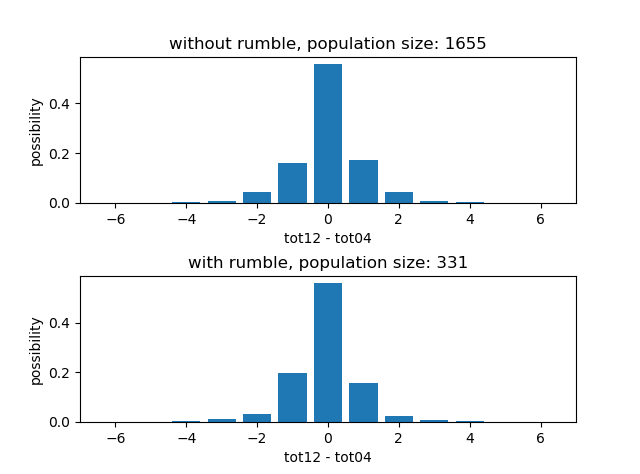
\includegraphics[width=0.5\textwidth]{with-and-without-rumble-diff.png}
    \caption{distribution of $tot12-tot04$ on roads with and without rumble treatment}
    \label{fig:general-effect}
\end{figure}

We then consider the roads of large curvature. We first check roads with curve degree greater than 3, the mean value of $tot12-tot04$ for the treat group is -0.077 against 0.108 for the control group, and the p value is 0.036, which rejects the null hypothesis. When we further increase the curve degree threshold to 5, the difference is more significant, with the mean value difference increase to 0.272 and p value decrease to 0.028. Figure ~\ref{fig:curve-grt3} and figure ~\ref{fig:curve-grt5} shows the distribution of $tot12-tot04$ of the two cases respectively. 

\begin{figure}[H]
    \centering
    \begin{subfigure}{.5\textwidth}
        \centering
        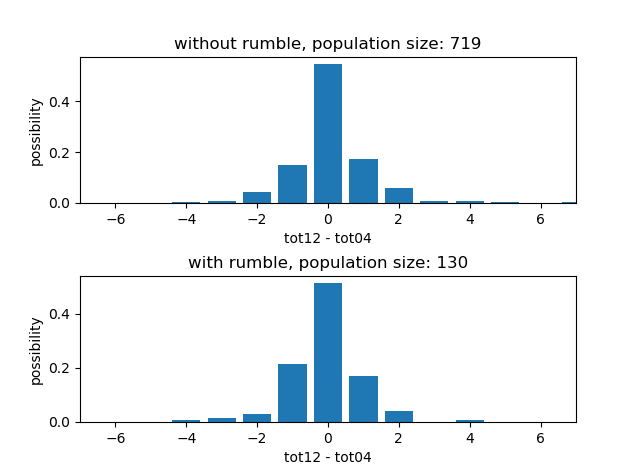
\includegraphics[width=1\textwidth]{with-and-without-rumble-curvature-grt3-diff.png}
        \caption{distribution of $tot12-tot04$ on roads of curve degree $>$ 3     with and without rumble treatment}
        \label{fig:curve-grt3}
    \end{subfigure}%
    \begin{subfigure}{.5\textwidth}
        \centering
        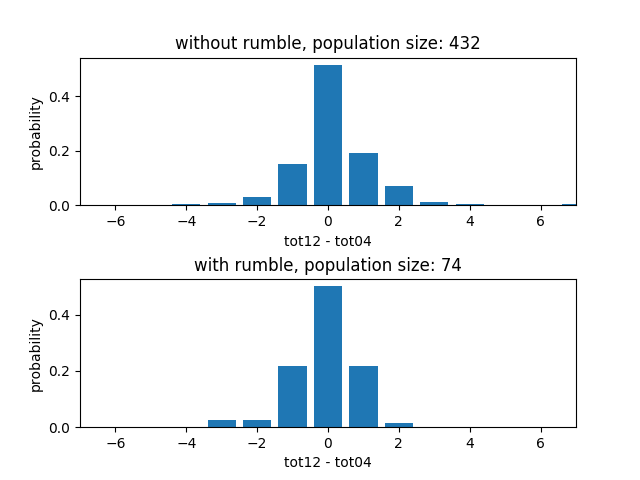
\includegraphics[width=1\textwidth]{with-and-without-rumble-curvature-grt5-diff.png}
        \caption{distribution of $tot12-tot04$ on roads of curve degree $>$ 5     with and without rumble treatment}
        \label{fig:curve-grt5}
    \end{subfigure}
\end{figure}

The second road feature in this study is the posted speed limit. The speed limit in this dataset has two categories, i.e. smaller than 45 mph and greater than 45 mph. We expect that car accidents tend to happen more frequently on roads with higher speed limit and rumble stirps could help to reduce the chance. Indeed, the mean value of $tot12-tot04$ for the treat group is again smaller than the control group (-0.104 versus 0.047), the p value, however, is 0.059, which is a little bit higher than $alpha$. Figure ~\ref{fig:speed} presents the distribution of $tot12-tot04$ for the two groups.

\begin{figure}[h!]
    \centering
    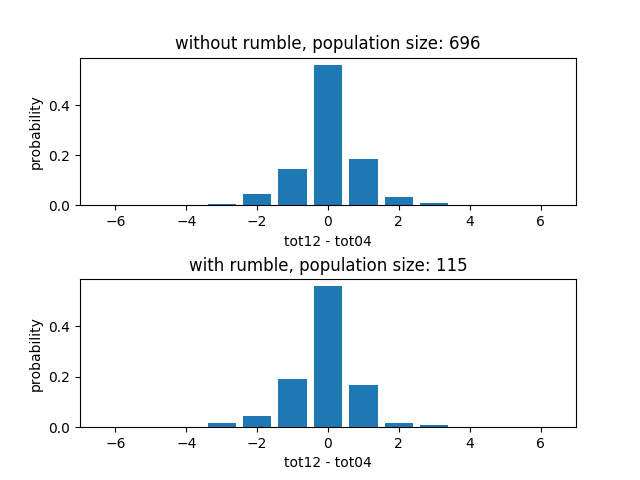
\includegraphics[width=0.5\textwidth]{with-and-without-rumble-speed-grt45-diff.png}
    \caption{distribution of $tot12-tot04$ on roads of speed limit greater than 45 mph with and without rumble treatment}
    \label{fig:speed}
\end{figure}

The last road feature we pick out is road width. Road width is categorized into 3 values in this dataset. More specifically, they are "$<=$ 20", :1, "$>$ 20 and $<$ 24" and "$>=$ 24", with feet being the unit.  While we suspected that a narrower road tends to be more dangerous, the test does not produce a positive result for the rumbles strips' effectiveness on roads in the "$<=$ 20" category, as the mean value of the treat group is 0.1 while the control group has a small mean value of 0.087. Interestingly, when we further check the widest road category, we see a positive result. The mean value in this case is -1.891 for the treat group and 0.006 for the other, with the p value being 0.029. As show in figure ~\ref{fig:width-cat0} and figure ~\ref{fig:width-cat2}, it's noticeable that the distribution of $tot12-tot04$ is much higher at value -1 with rumble strips installation. 

\begin{figure}[H]
    \centering
    \begin{subfigure}{.5\textwidth}
        \centering
        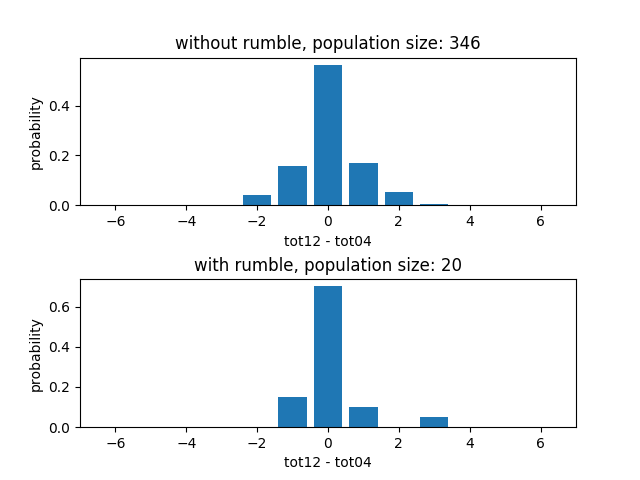
\includegraphics[width=1\textwidth]{with-and-without-rumble-width-cat0-diff.png}
        \caption{distribution of $tot12-tot04$ on roads of curve degree $>$ 3     with and without rumble treatment}
        \label{fig:width-cat0}
    \end{subfigure}%
    \begin{subfigure}{.5\textwidth}
        \centering
        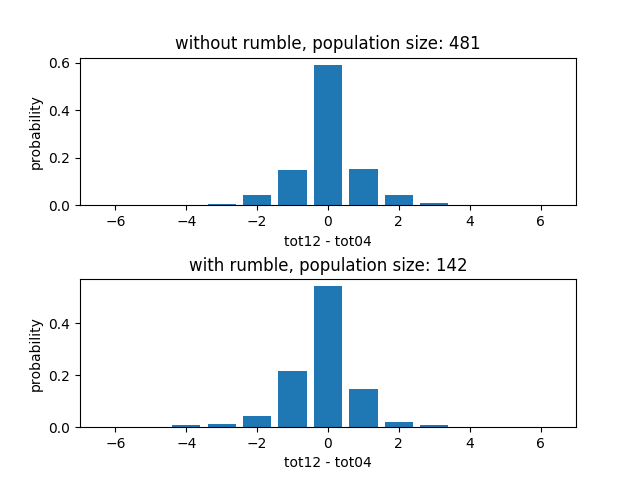
\includegraphics[width=1\textwidth]{with-and-without-rumble-width-cat2-diff.png}
        \caption{distribution of $tot12-tot04$ on roads of curve degree $>$ 5     with and without rumble treatment}
        \label{fig:width-cat2}
    \end{subfigure}
\end{figure}

To further study the reason that rumble strips show a better result in wider roads, we plot a scatter plot of road width against AADT as shown in figure ~\ref{fig:width-adt}. We see that a more spacious road is more likely to carry more traffics, and thus higher probability of crashes, which makes the effects of rumble strips, if any, more prominent.

\begin{figure}[h!]
    \centering
    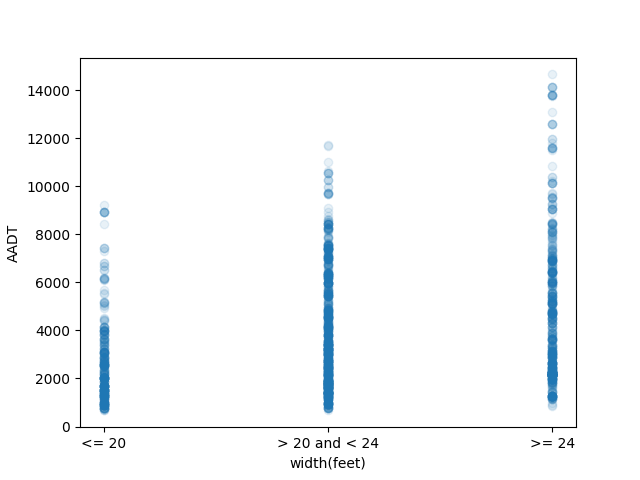
\includegraphics[width=0.5\textwidth]{width-adt-scatter.png}
    \caption{scatter plot for traffic volume versus width}
    \label{fig:width-adt}
\end{figure}

\section*{Conclusion}

In this study, we explore the effectiveness of rumble strips by comparing the changes in yearly car crashes number between roads with and without rumble installed under different road conditions, and there are positive results in most of the examined cases. When we compare the $tot12-tot04$ distribution between the treat group and the control group, we find that without rumble strips installation, the value at 1 is tends to be higher then the value at -1, while it's the other way around on roads with rumble stripes installation, which means rumble strips indeed have some positive effects in reducing crashes. And according the cases we have studied, the effects varies across roads with different conditions.

\bibliography{project2} 
\bibliographystyle{ieeetr}
\end{document}

